\documentclass[14pt]{extarticle}
\usepackage[utf8]{inputenc}
\usepackage[T1]{fontenc}
\usepackage[spanish,es-lcroman]{babel}
\usepackage{amsmath}
\usepackage{amsthm}
\usepackage{physics}
\usepackage{tikz}
\usepackage{float}
\usepackage[autostyle,spanish=mexican]{csquotes}
\usepackage[per-mode=symbol]{siunitx}
\usepackage{gensymb}
\usepackage{multicol}
\usepackage{enumitem}
\usepackage[left=2.00cm, right=2.00cm, top=2.00cm, 
     bottom=2.00cm]{geometry}

\usepackage{Estilos/ColoresLatex}
\usepackage{makecell}

\newcommand{\textocolor}[2]{\textbf{\textcolor{#1}{#2}}}
%\renewcommand{\questionlabel}{\thequestion)}
\decimalpoint
\sisetup{bracket-numbers = false}

\title{\vspace*{-2cm} Ejercicios de Velocidad \\  Solución - Física III\vspace{-5ex}}
\date{}

\begin{document}
\maketitle

\section*{Ejercicios a resolver.}

\begin{enumerate}
\item ¿A qué distancia (en metros) viaja hacia adelante un automóvil que se mueve a razón de 55 millas/h durante \SI{1}{\second} de tiempo, que es lo que le toma ver un accidente al lado de la carretera?

Como la velocidad está en millas/h hacemos la conversión a metros por segundo, ocupando los siguientes factores:

1 milla = \SI{1609}{\meter} \\
\SI{1}{\hour} = \SI{3600}{\second}
\begin{align*}
v = 55 \, \dfrac{\text{millas}}{h} \left( \dfrac{\SI{1609}{\meter}}{1 \, \text{milla}} \right)\left( \dfrac{\SI{1}{\hour}}{\SI{3600}{\second}} \right) = \dfrac{\SI{88495}{\meter}}{\SI{3600}{\second}} = \SI[per-mode=fraction]{24.58}{\meter\per\second}
\end{align*}

\begin{minipage}[t]{0.4\linewidth}
\textocolor{red}{1. Datos:}
\begin{align*}
v &= 55 \, \text{millas/h} = \SI[per-mode=fraction]{24.58}{\meter\per\second} \\
t &= \SI{1}{\second} \\
d &= \, ?
\end{align*}
\end{minipage}
\hspace{1cm}
\begin{minipage}[t]{0.4\linewidth}
\textocolor{red}{2. Expresión:}
\begin{align*}
v = \dfrac{d}{t} \hspace{0.2cm} \Rightarrow \hspace{0.2cm} d = v \, t
\end{align*}
\end{minipage}

\textocolor{red}{3. Sustitución:}
\begin{align*}
d = \left( \SI[per-mode=fraction]{24.58}{\meter\per\second} \right) (\SI{1}{\second}) = \SI{24.58}{\meter}
\end{align*}
\item El lanzador de los Medias Rojas de Boston, Roger Clemens, lanzó una bola rápida a una velocidad horizontal de \SI{160}{\kilo\meter\per\hour}, según fue verificado con una pistola de radar. ¿Qué tanto le tomó a la bola llegar a la base de meta, que está a una distancia de \SI{18.4}{\meter}?

Para tener un manejo consistente de unidades, pasamos los \SI{160}{\kilo\meter\per\hour} a \unit{\meter\per\second}
\begin{align*}
\SI[per-mode=fraction]{160}{\kilo\meter\per\hour} \left( \dfrac{\SI{1000}{\meter}}{\SI{1}{\kilo\meter}} \right) \left( \dfrac{\SI{1}{\hour}}{\SI{3600}{\second}} \right) = \SI[per-mode=fraction]{44.44}{\meter\per\second}
\end{align*}

\begin{minipage}[t]{0.4\linewidth}
\textocolor{red}{1. Datos:}
\begin{align*}
v &= \SI[per-mode=fraction]{160}{\kilo\meter\per\hour} = \SI[per-mode=fraction]{44.44}{\meter\per\second} \\
d &= \SI{18.4}{\meter} \\
t &= \, ?
\end{align*}
\end{minipage}
\hspace{1cm}
\begin{minipage}[t]{0.4\linewidth}
\textocolor{red}{2. Expresión:}
\begin{align*}
v = \dfrac{d}{t} \hspace{0.2cm} \Rightarrow \hspace{0.2cm} t = \dfrac{d}{v}
\end{align*}
\end{minipage}

\textocolor{red}{3. Sustitución:}
\begin{align*}
t =  \dfrac{\SI{18.4}{\meter}}{\displaystyle \SI[per-mode=fraction]{44.44}{\meter\per\second}} = \SI{0.414}{\second}
\end{align*}

Revisa que las unidades son segundos, ya que:
\begin{align*}
\dfrac{\unit{\meter}}{\displaystyle \unit[per-mode=fraction]{\meter\per\second}} = \dfrac{\displaystyle \dfrac{\unit{\meter}}{1}}{\displaystyle \unit[per-mode=fraction]{\meter\per\second}} = \dfrac{\unit{\meter\second}}{\unit{\meter}} = \unit{\second}
\end{align*}
\item ¿A qué velocidad promedio iba un auto que recorrió \SI{250}{\kilo\meter} en \SI{3}{\hour}?

Revisemos que las unidades de la distancia están en \unit{\kilo\meter} y el tiempo en \unit{hour}, por lo que las llevamos a las unidades fundamentales del Sistema Internacional, es decir: metros y segundos, respectivamente:
\begin{align*}
\SI{250}{\kilo\meter} &\left( \dfrac{\SI{1000}{\meter}}{\SI{1}{\kilo\meter}} \right) = \SI{2.5d5}{\meter} \\[0.5em]
\SI{3}{\hour} &\left( \dfrac{\SI{3600}{\second}}{\SI{1}{\hour}} \right) = \SI{1.08d4}{\second}
\end{align*}

\begin{minipage}[t]{0.4\linewidth}
\textocolor{red}{1. Datos:}
\begin{align*}
d &= \SI{2.5d5}{\meter} \\
t &= \SI{1.08d4}{\second} \\
v &= \, ?
\end{align*}
\end{minipage}
\hspace{1cm}
\begin{minipage}[t]{0.4\linewidth}
\textocolor{red}{2. Expresión:}
\begin{align*}
v = \dfrac{d}{t}
\end{align*}
\end{minipage}

\textocolor{red}{3. Sustitución:}
\begin{align*}
v = \dfrac{\SI{2.5d5}{\meter}}{\SI{1.08d4}{\second}} = \SI[per-mode=fraction]{23.14}{\meter\per\second}
\end{align*}
\item ¿A qué velocidad en \unit{\kilo\meter\per\hour} corrió Usain Bolt en el Campeonato Mundial de Berlín en el año 2009 para batir el récord mundial de los \SI{100}{\meter} planos en \SI{9.58}{\second}?

Primero encontramos la velocidad en metros por segundo del corredor:

\begin{minipage}[t]{0.4\linewidth}
\textocolor{red}{1. Datos:}
\begin{align*}
d &= \SI{100}{\meter} \\
t &= \SI{9.58}{\second} \\
v &= \, ?
\end{align*}
\end{minipage}
\hspace{1cm}
\begin{minipage}[t]{0.4\linewidth}
\textocolor{red}{2. Expresión:}
\begin{align*}
v = \dfrac{d}{t}
\end{align*}
\end{minipage}

\textocolor{red}{3. Sustitución:}
\begin{align*}
v = \dfrac{\SI{100}{\meter}}{\SI{9.58}{\second}} = \SI[per-mode=fraction]{10.43}{\meter\per\second}
\end{align*}

Como nos pide el enunciado expresar la velocidad en \unit{\kilo\meter\per\hour}, hacemos la conversión de unidades:
\begin{align*}
v = \SI[per-mode=fraction]{10.43}{\meter\per\second} \left( \dfrac{\SI{1}{\kilo\meter}}{\SI{1000}{\meter}} \right) \left( \dfrac{\SI{3600}{\second}}{\SI{1}{\hour}} \right) = \dfrac{\SI{37548}{\kilo\meter}}{\SI{1000}{\hour}} = \SI[per-mode=fraction]{37.54}{\kilo\meter\per\hour}
\end{align*}
\item ¿Qué distancia recorrió un avión que viajaba a \SI{750}{\kilo\meter\per\hour} después de \SI{2.5}{\hour} de vuelo?

Es importante revisar las unidades que se nos indican en el enunciado, las debemos de llevar siempre a las unidades fundamentales del Sistema Internacional:

\begin{align*}
\SI[per-mode=fraction]{750}{\kilo\meter\per\hour} &\left( \dfrac{\SI{1000}{\meter}}{\SI{1}{\kilo\meter}} \right) \left( \dfrac{\SI{1}{\hour}}{\SI{3600}{\second}} \right) = \dfrac{\SI{7.5d5}{\meter}}{\SI{3.6d3}{\second}} = \SI[per-mode=fraction]{208.33}{\meter\per\second} \\[0.5em]
\SI{2.5}{\hour} &\left( \dfrac{\SI{3600}{\second}}{\SI{1}{\hour}} \right) = \SI{9d3}{\second}
\end{align*}

\begin{minipage}[t]{0.4\linewidth}
\textocolor{red}{1. Datos:}
\begin{align*}
v &= \SI[per-mode=fraction]{208.33}{\meter\per\second} \\
t &= \SI{9d3}{\second} \\
d &= \, ?
\end{align*}
\end{minipage}
\hspace{1cm}
\begin{minipage}[t]{0.4\linewidth}
\textocolor{red}{2. Expresión:}
\begin{align*}
v = \dfrac{d}{t} \hspace{0.2cm} \Rightarrow \hspace{0.2cm} d = v \, t
\end{align*}
\end{minipage}

\textocolor{red}{3. Sustitución:}
\begin{align*}
d = \left( \SI[per-mode=fraction]{208.33}{\meter\per\second} \right) \left( \SI{9d3}{\second} \right) = \SI{1.87497d6}{\meter} = \SI{1874.97}{\kilo\meter}
\end{align*}
\item Calcula la velocidad en \unit{\kilo\meter\per\hour}, a la que corrió el atleta keniata Wilson Kipsang Kiprotich para batir el récord mundial vigente, que realizó en el maratón de Berlín, en el año 2013, cuya distancia total es de \SI{42.195}{\kilo\meter}, en un tiempo de \SI{2}{\hour} \SI{3}{\minute} \SI{23}{\second}.

Hay que calcular el tiempo total en horas, es decir, pasar los minutos y segundos a horas:
\begin{align*}
t &= \SI{2}{\hour} \, \SI{3}{\minute} \, \SI{23}{\second} = \SI{2}{\hour} + (\SI{3}{\minute}) \left( \dfrac{\SI{1}{\hour}}{\SI{60}{\minute}} \right) + (\SI{23}{\second}) \left( \dfrac{\SI{1}{\hour}}{\SI{3600}{\second}} \right) = \\[0.5em]
t &= \SI{2}{\hour} + \SI{0.05}{\hour} + \SI{6.38d-3}{\hour} = \\[0.5em]
t &= \SI{2.05638}{\hour}
\end{align*}

\begin{minipage}[t]{0.4\linewidth}
\textocolor{red}{1. Datos:}
\begin{align*}
d &= \SI{42.195}{\kilo\meter} \\
t &= \SI{2.05638}{\hour} \\
v &= \, ?
\end{align*}
\end{minipage}
\hspace{1cm}
\begin{minipage}[t]{0.4\linewidth}
\textocolor{red}{2. Expresión:}
\begin{align*}
v = \dfrac{d}{t}
\end{align*}
\end{minipage}

\textocolor{red}{3. Sustitución:}
\begin{align*}
v = \dfrac{\SI{42.195}{\kilo\meter}}{\SI{2.05638}{\hour}} = \SI[per-mode=fraction]{20.51}{\kilo\meter\per\hour}
\end{align*}
    
\item En la siguiente gráfica se muestra el desplazamiento en función del tiempo para cierto objeto que se mueve a lo largo del eje $x$.
\begin{figure}[H]
    \centering
    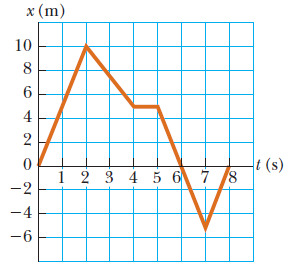
\includegraphics[scale=1]{Imagenes/Ejercicio_Cuenta_01.png}
\end{figure}
Como tenemos valores de posición y de tiempo en los intervalos, ocupamos la expresión para la velocidad:
\begin{align*}
v = \dfrac{\Delta \, y}{\Delta \, x} = \dfrac{y_{f} - y_{i}}{x_{f} - x_{i}}
\end{align*}

Encuentra la velocidad en los siguientes intervalos de tiempo:
\begin{enumerate}[label=\alph*)]
\item \num{0} a \SI{2}{\second}
\begin{align*}
v = \dfrac{y_{f} - y_{i}}{x_{f} - x_{i}} = \dfrac{\SI{10}{\meter} - \SI{0}{\meter}}{\SI{2}{\second} - \SI{0}{\second}} = \dfrac{\SI{10}{\meter}}{\SI{2}{\second}} = \SI[per-mode=fraction]{5}{\meter\per\second}
\end{align*}
\item \num{0} a \SI{4}{\second}
\begin{align*}
v = \dfrac{y_{f} - y_{i}}{x_{f} - x_{i}} = \dfrac{\SI{5}{\meter} - \SI{0}{\meter}}{\SI{4}{\second} - \SI{0}{\second}} = \dfrac{\SI{5}{\meter}}{\SI{4}{\second}} = \SI[per-mode=fraction]{1.25}{\meter\per\second}
\end{align*}  
\item \num{2} a \SI{4}{\second}
\begin{align*}
v = \dfrac{y_{f} - y_{i}}{x_{f} - x_{i}} = \dfrac{\SI{5}{\meter} - \SI{10}{\meter}}{\SI{4}{\second} - \SI{2}{\second}} = \dfrac{- \SI{5}{\meter}}{\SI{2}{\second}} = -\SI[per-mode=fraction]{2.5}{\meter\per\second}
\end{align*}
\item \num{4} a \SI{7}{\second}
\begin{align*}
v = \dfrac{y_{f} - y_{i}}{x_{f} - x_{i}} = \dfrac{-\SI{5}{\meter} - \SI{5}{\meter}}{\SI{7}{\second} - \SI{3}{\second}} = \dfrac{-\SI{10}{\meter}}{\SI{4}{\second}} = -\SI[per-mode=fraction]{2.5}{\meter\per\second}
\end{align*}
\item \num{0} a \SI{8}{\second}
\begin{align*}
v = \dfrac{y_{f} - y_{i}}{x_{f} - x_{i}} = \dfrac{\SI{0}{\meter} - \SI{0}{\meter}}{\SI{8}{\second} - \SI{0}{\second}} = \dfrac{\SI{0}{\meter}}{\SI{8}{\second}} = \SI[per-mode=fraction]{0}{\meter\per\second}
\end{align*}
\end{enumerate}
\item Un motociclista adquiere una velocidad de \SI{50}{\kilo\meter\per\hour} en \SI{6}{\second}. ¿Cuál es su aceleración en \unit{\meter\per\square\second}?

Convertimos la velocidad de \SI{50}{\kilo\meter\per\hour} a \unit{\meter\per\second}:
\begin{align*}
\SI[per-mode=fraction]{50}{\kilo\meter\per\hour} \left( \dfrac{\SI{d3}{\meter}}{\SI{1}{\kilo\meter}} \right) \left( \dfrac{\SI{1}{\hour}}{\SI{3.6d2}{\second}} \right) = \SI[per-mode=fraction]{13.88}{\meter\per\second}
\end{align*}
\begin{minipage}[t]{0.4\linewidth}
\textocolor{red}{1. Datos:}
\begin{align*}
v_{0} &= \SI{0}{\kilo\meter\per\hour} \\
v_{f} &= \SI{50}{\kilo\meter\per\hour} = \SI[per-mode=fraction]{13.88}{\meter\per\second}\\
t &= \SI{6}{\second} \\
a &= \, ?
\end{align*}
\end{minipage}
\hspace{1cm}
\begin{minipage}[t]{0.4\linewidth}
\textocolor{red}{2. Expresión:}
\begin{align*}
a = \dfrac{v_{f} - v_{i}}{t}
\end{align*}
\end{minipage}

\textocolor{red}{3. Sustitución:}
\begin{align*}
a = \dfrac{\displaystyle \SI[per-mode=fraction]{13.88}{\meter\per\second} - \SI[per-mode=fraction]{0}{\meter\per\second}}{\SI{6}{\second}} = \SI[per-mode=fraction]{2.31}{\meter\per\square\second}
\end{align*}
\item Un camión lleva una velocidad inicial de \SI{6}{\meter\per\second}, a los \SI{4}{\second} su velocidad es de \SI{8}{\meter\per\second}. Calcula su aceleración.

\begin{minipage}[t]{0.4\linewidth}
\textocolor{red}{1. Datos:}
\begin{align*}
v_{0} &= \SI{6}{\meter\per\second} \\
v_{f} &= \SI{8}{\meter\per\second}\\
t &= \SI{4}{\second} \\
a &= \, ?
\end{align*}
\end{minipage}
\hspace{1cm}
\begin{minipage}[t]{0.4\linewidth}
\textocolor{red}{2. Expresión:}
\begin{align*}
a = \dfrac{v_{f} - v_{i}}{t}
\end{align*}
\end{minipage}

\textocolor{red}{3. Sustitución:}
\begin{align*}
a = \dfrac{\displaystyle \SI[per-mode=fraction]{8}{\meter\per\second} - \SI[per-mode=fraction]{6}{\meter\per\second}}{\SI{4}{\second}} = \SI[per-mode=fraction]{0.5}{\meter\per\square\second}
\end{align*}
\item  Un avión vuela en la misma dirección y sentido a \SI{860}{\kilo\meter\per\hour} durante un tiempo de \SI{20}{\minute}. ¿Cuál es su aceleración durante ese intervalo de tiempo y por qué?

Para ser consistentes con nuestro manejo de unidades, convertimos \SI{860}{\kilo\meter\per\hour} a \unit{\meter\per\second} y el tiempo \SI{20}{\minute} a \unit{\second}:
\begin{align*}
\SI[per-mode=fraction]{860}{\kilo\meter\per\hour} & \left( \dfrac{\SI{d3}{\meter}}{\SI{1}{\kilo\meter}} \right) \left( \dfrac{\SI{1}{\hour}}{\SI{3.6d2}{\second}} \right) = \SI[per-mode=fraction]{51.66}{\meter\per\second} = \\[0.5em]
\SI{20}{\minute} &\left( \dfrac{\SI{60}{\second}}{\SI{1}{\minute}} \right) = \SI{1.2d3}{\second}
\end{align*}

\begin{minipage}[t]{0.4\linewidth}
\textocolor{red}{1. Datos:}
\begin{align*}
v_{0} &= \SI{860}{\kilo\meter\per\hour} = \SI[per-mode=fraction]{51.66}{\meter\per\second} \\[0.5em]
v_{f} &= \SI{860}{\kilo\meter\per\hour} = \SI[per-mode=fraction]{51.66}{\meter\per\second} \\[0.5em]
t &= \SI{20}{\minute} = \SI{1.2d3}{\second} \\[0.5em]
a &= \, ?
\end{align*}
\end{minipage}
\hspace{1cm}
\begin{minipage}[t]{0.4\linewidth}
\textocolor{red}{2. Expresión:}
\begin{align*}
a = \dfrac{v_{f} - v_{i}}{t}
\end{align*}
\end{minipage}

\textocolor{red}{3. Sustitución:}
\begin{align*}
a = \dfrac{\displaystyle \SI[per-mode=fraction]{51.66}{\meter\per\second} - \SI[per-mode=fraction]{51.66}{\meter\per\second}}{\SI{1.2d3}{\second}} = \SI[per-mode=fraction]{0}{\meter\per\square\second}
\end{align*}
Encontramos que la aceleración del avión es cero durante ese intervalo de tiempo, ya que no cambia su velocidad. Notemos que aunque la aceleración es cero, el objeto mantiene una velocidad constante.
\end{enumerate}


\end{document}